\begin{song}{title=\predtitle \centering Slunečný hrob \\\large Blue Effect  \vspace*{--0.0cm}}  %% sem se napíše jméno songu a autor
\velky
\begin{centerjustified}

\ssloka{Rec:} Usínám a chtěl bych se vrátit o nějakej ten rok zpátky,

bejt zase malým klukem, kterej si rád hraje a který je s tebou.

\sloka
^{E\z }Zdá se ^{F^{\#}mi}mi, ^{G^{\#}mi}je~to ^{\z F^{\#}mi}moc~let,

já byl kluk, kterej chtěl

znáti svět, s tebou jsem si hrál.

\sloka
Vrátím se a chtěl bych rád

být s tebou, zavzpomínat,

^{E}mám tu ^{\z F^{\#}mi}teď ^{G^{\#}mi}ale ^{\z F^{\#}mi}zprávu ^{\z E}zlou. ^{E7}

\refren
^{C^{\#}mi \z}Su -- ^{\z D^{\#}mi}chá ^{A \z}hlína ^{G^{\#}mi \z}ta -- ^{F^{\#}mi}dy,

^{C^{\#}mi \z}bez ^{D^{\#}mi \z}kví -- ^{A}tí, bez ^{G^{\#}mi}vo -- ^{F^{\#}mi}dy,

^{G^{\#}mi}já na ni ^{F^{\#}mi \z}poklekám,

^{G^{\#}mi \z}vzpomínkou ^{\z H}pocta se vzdává.

\sloka
Loučím se a něco však

tam zůstalo z těch našich dnů,

já teď vím, věrný zůstanu.


\ssloka{Rec:} Nemohu spát, probouzím se a zase se nemohu ubránit myšlence,

vrátit se o nějakej ten rok zpátky, bejt zase malým klukem,

který si rád hraje, který je s tebou.

\end{centerjustified}

\centering
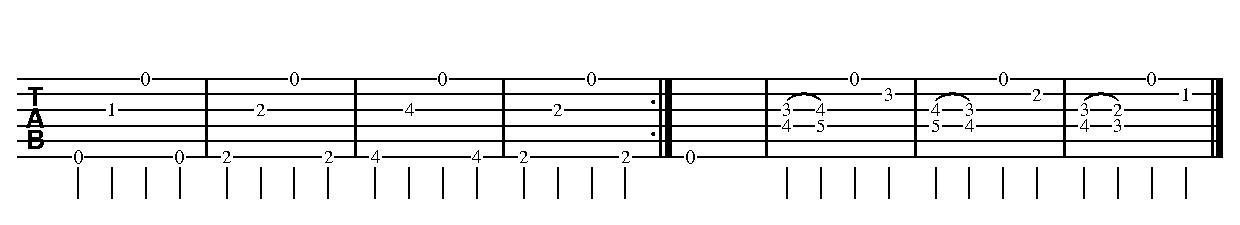
\includegraphics[scale=\defaulttabscale]{../taby/slunecnyhrob.pdf}

\setcounter{Slokočet}{0}
\end{song}


